\documentclass[12pt]{article}

\usepackage{amssymb,amsmath,amsthm} % Include AMS Math symbols
\usepackage{graphicx}               % Allows for importation of figures 

\usepackage{booktabs} % professional table typesetting commands 

\usepackage{color}   % Sets up a nice typesetting environment for Python
\usepackage{float} %  added to put my tabel right where I want it
\usepackage{listings}
\definecolor{dkgreen}{rgb}{0,0.6,0}
\definecolor{gray}{rgb}{0.5,0.5,0.5}
\definecolor{mauve}{rgb}{0.58,0,0.82}
\lstset{frame=tb,
  language=Python,
  aboveskip=3mm,
  belowskip=3mm,
  showstringspaces=false,
  columns=flexible,
  basicstyle={\small\ttfamily},
  numbers=left,
  numberstyle=\tiny\color{gray},
  keywordstyle=\color{blue},
  commentstyle=\color{dkgreen},
  stringstyle=\color{mauve},
  breaklines=true,
  breakatwhitespace=true,
  tabsize=3
}

% define command \expandableinput  for table input
\makeatletter
\def\expinput#1{\@@input#1 }
\makeatother

\title{ HW \#3 \\ Math/CS 471, Fall 2026}
\author{Theo Nichols \\ Andrew Vargas}
\date{October 6th, 2026}   % Activate to display a given date or no date


\begin{document}

% Display title
\maketitle
\clearpage

\section{Comparison of 1D Integration Rules}

\subsection{Trapezoidal Rule}

\subsubsection{Overview}
We are tasked with approximating the value of the integral
\begin{equation}
I = \int_{-1}^{1} e^{\cos(kx)}\,dx, \text{ With } k=\pi,\quad k=\pi^2
\end{equation}
We are asked to compare the performance of two different methods. That is, the trapezoidal rule and Gaussian quadrature. The trapezoid rule is defined as \\
\begin{equation}
\int_a^b f(x) \, dx \approx h \left[ \frac{f(a) + f(b)}{2} + \sum_{i=1}^{n-1} f(x_i) \right]
\end{equation}
where a and b are the beginning and end of our first interval respectively, h is the width of our interval or our step size, and n is the number of subintervals. 
\\We begin by determining the rate at which the absolute value of our error estimate decreases as the number of subintervals increases. That is, how does 
\begin{equation}
    error \approx |I_{n+1} - I_n|
\end{equation}
decrease as we increase the number of intervals, where $I_n, \space I_{n+1}$ refer to our approximation of I at n and n+1 subintervals. We will also use this error approximation to determine the number of subintervals such that the difference between successive iterations is within a prescribed tolerance, $10^{-10}$. We will then plot these values against linear, quadratic, cubic and exponential reference functions to extrapolate a rate of convergence. It should be noted that our error estimate is a local error, as we do not know the true value of I, but merely the difference between successive iterations of the method.
\\


\subsubsection{Method}

Implementing trapezoid rule was fairly straightforward, requiring only a few lines of Python.
\begin{lstlisting}
def trapezoid(func, k, n):
  interval = np.linspace(-1, 1, n+1)
  h = 2 / n
  fVals = func(k, interval)
  return h * ( ((fVals[0] + fVals[-1]) / 2) + np.sum(fVals[1:-1]))
\end{lstlisting}


This function was then called and the results stored in lists for later use. To calculate the error between successive intervals, we simply calculated the absolute value of the difference between our current iteration and the last. Once the program found a value for n that yielded an error estimate less than the tolerance, we logged this to the console and broke out of the loop.
Below is the result of comparing our error to the number of subintervals.


\begin{figure}[htb]
\begin{center}
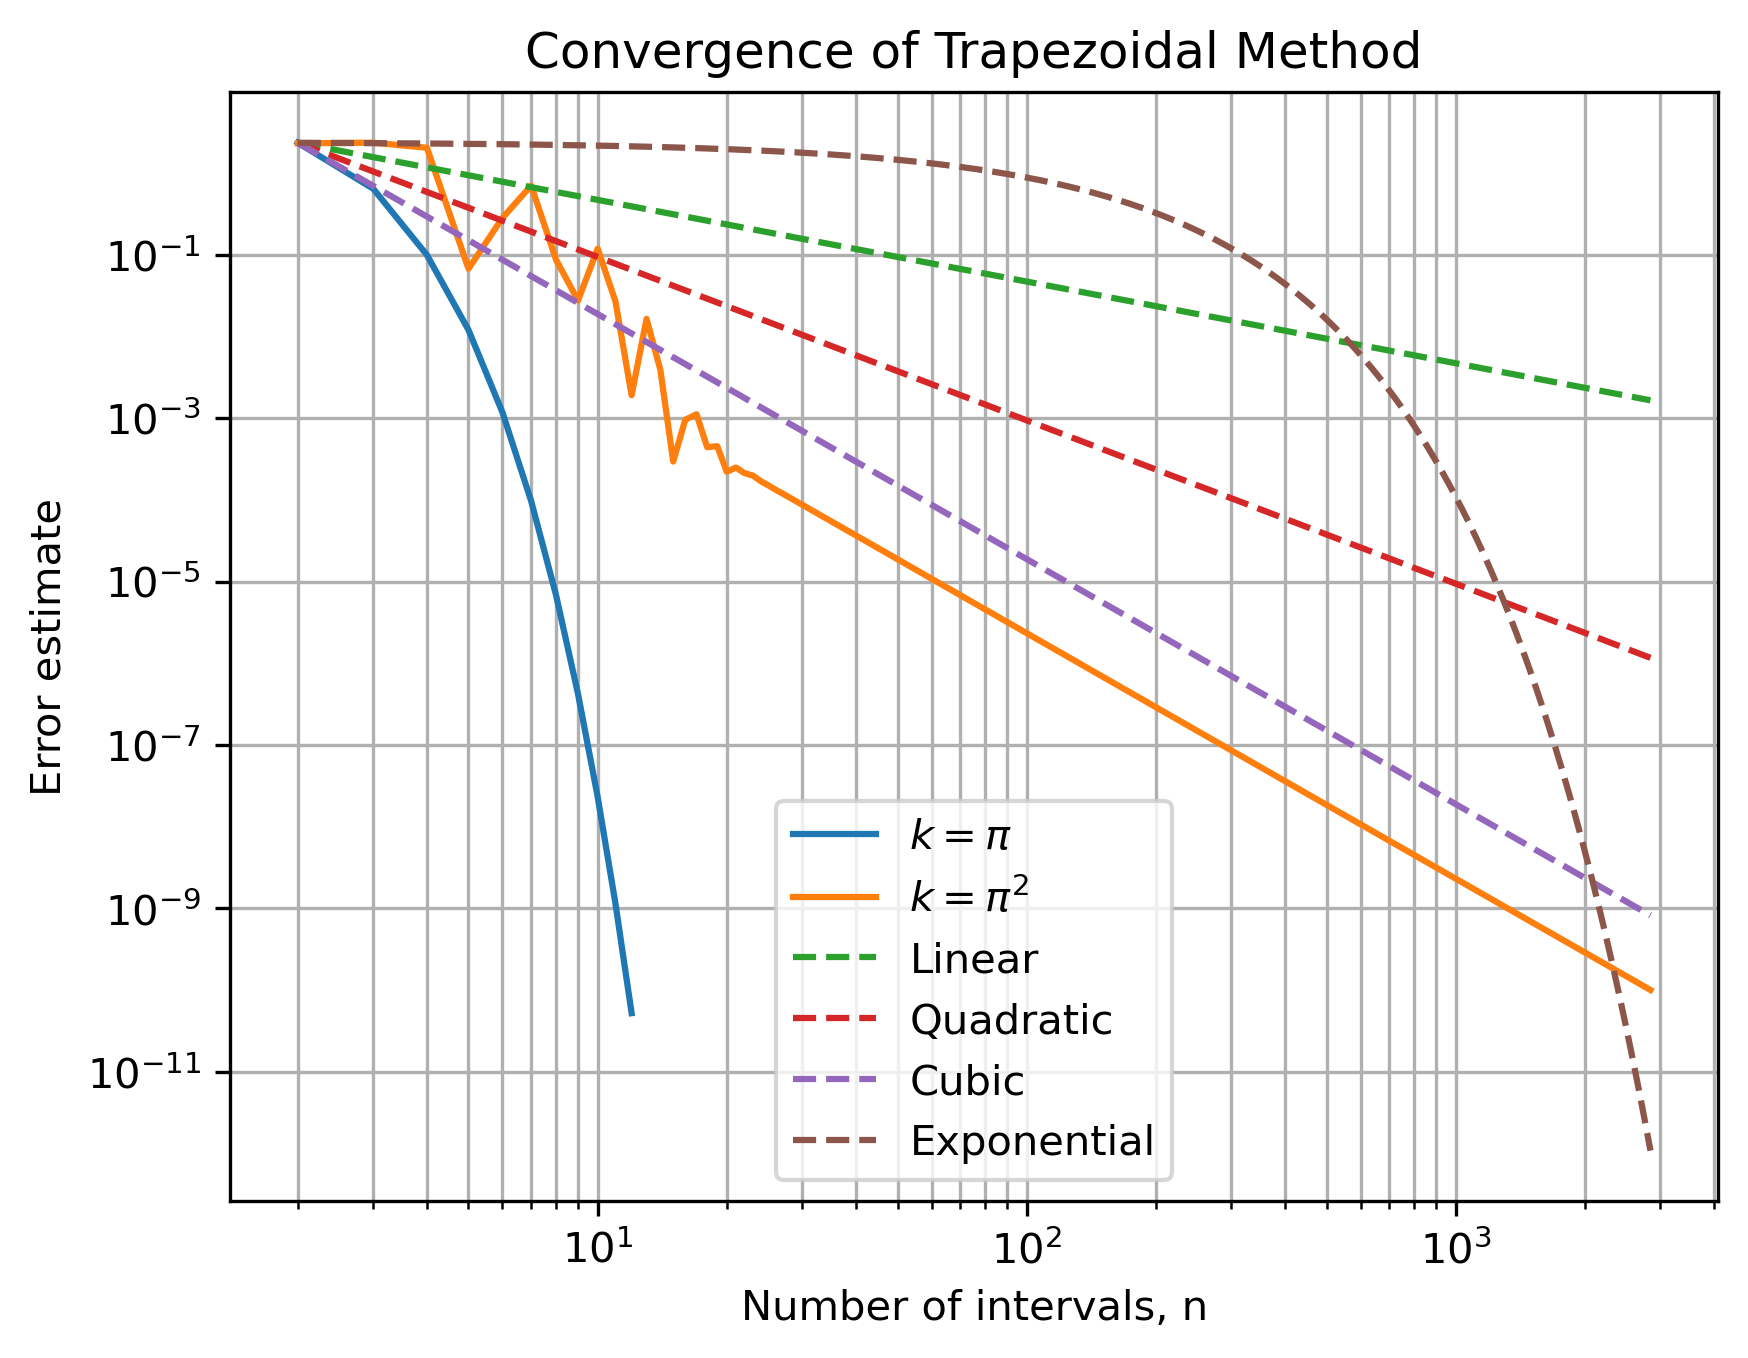
\includegraphics[width=0.75\textwidth]{trapezoidal_convergence.png}
   \caption{Relation of Error Estimate and Number of Subintervals in Trapezoid Rule (\ref{eq:overcomplicated_exp_function}).}
    \label{fig:1}
\end{center}
\end{figure}

As can be seen above, when $k=\pi^2$, the convergence appears roughly quadratic or even cubic. However, interestingly, when $k=\pi$, the method appears to converge much more rapidly.

\\

\subsubsection{Interpretation} 
The quadratic rate of convergence was not surprising for the $k=\pi^2$ case, as this aligns with the convergence rate derived in class. The $k=\pi$ case was surprising, because the method appears to converge more rapidly than any of the reference curves. Something interesting to note, is that the period of $e^{cos(\pi x)}$ is two, which is exactly the length of the interval we are integrating over. Whereas for $e^{cos(\pi^2 x)}$, the period is $\frac{2}{\pi}$. There is perhaps a relation between this fact and the observed convergence, but at present we do not have an explanation for the more rapid convergence of the trapezoid rule in this case.

\newpage
\subsection{Gaussian Quadrature}

\subsubsection{Overview}
Next, we approximate the same integral of
\begin{equation}
    I = \int_{-1}^{1}e^{cos(kx)}dx, k = \pi, k = \pi^2,
\end{equation}
using Gaussian Quadrature. \\\\
Unlike the Trapezoidal Rule, which evaluates the integrand at equally spaced points, Gaussian Quadrature uses specially selected quadrature nodes $x_i$ and corresponding weights $\omega_i$.\\\\ 
Nodes and weights are chosen so that the integral can be approximated using a relatively small number of function evaluations. \\\\
For this assignment, the weight function is $w(x) = 1$, and the Gauss Quadrature takes the form of approximately \begin{equation}
    I_n \approx \sum_{i=0}^{n}\omega_if(x_i).
\end{equation}
We used the provided lglnodes(n) function to the required nodes and weights. 
As with the trapezoidal rule, we compute approximations for increasing values of $n$ and use the difference between two successive approximations as an estimate of error, \begin{equation}
    (\delta_{abs})_n = |I_n - I_{n-1}|.
\end{equation}
The calculation is continued until this estimate falls below the assignment prescribed tolerance of \begin{equation}
    10^{-10}.
\end{equation}
The error estimates are plotted against the quadrature order n using log scales on bothe axes. Gauss quadrature is expected to show exponential convergence of the form \begin{equation}
    \epsilon(n) \sim C^{-\alpha n},
\end{equation}
so exponential reference curves are included in the convergence plot for comparison. 

\subsubsection{Method}
The Guass Quadratue method was implemented using the provide lglnodes(n) routine. For each quadrature order $n$, the routine returns $n + 1$ Legendre-Gauss-Lobatto nodes and their corresponding weights.\\\\
The integrand \begin{equation}
    f(x) = e^{cos(kx)}
\end{equation}
is evaluated at each of these nodes. Each function value is then multiplied by its correspond quadrature weight. \\\\
The resulting products are summed to obtained the approximation \begin{equation}
    I_n = \sum_{i=0}^{n}\omega_if(x_i).
\end{equation}
In the Python implementation, this calculation is performed by
\begin{lstlisting}
    def gauss(func, k, n):
    nodes, weights = lglnodes(n)
    fVals = func(k, nodes)
    return np.sum(weights * fVals)
\end{lstlisting}
The calculation is carried out separately for $k = \pi$ and $k = \pi^2$. Beginning with n = 2, the quadrature order is increased by one for each successive approximation. After both $I_n$ and the previous approximation $I_{n-1}$ are available, the error estimate is computed as 
\begin{equation}
    |I_n - I_{n-1}|.
\end{equation}
The iteration is stopped once this value is less than $10^{-10}$.\\\\
The error estimates for each value of $k$ are stored together with their corresponding quadrature orders and plotted on a log-log scale.\\\\
To compare the numerical results with the expected exponential convergence, reference curves of the form $C^{-\alpha n}$ are also plotted. In the implementation, $C = e$ is used and the value of $\alpha$ is adjusted experimentally so that the reference curves follow the observed decay of the numerical error.


\subsubsection{Interpretation}
Gauss Quadrature was applied to both $k = \pi$ and $k = \pi^2$. The iterations were continued until the difference between two successive approximations satisfied

\begin{equation}
    |I_n - I_{n-1}| < 10^{-10}.
\end{equation}
For $k = \pi$, the prescribed tolerance was reach at quadrature order n =20, producing \begin{equation}
    I_{20} \approx 2.532131755512648
\end{equation}
with an error estimate of \begin{equation}
    5.5278 \times 10^{-11}.
\end{equation}
For $k = \pi^2$, the tolerance was reached at $n = 54$, producing \begin{equation}
    I_{54} \approx 2.452283895120473
\end{equation}
with an error estimate of \begin{equation}
    6.7772 \times 10^{-11}.
\end{equation}

The convergence plots show that the error decreases rapidly as the quadrature order increases. The $k = \pi$ case decreases more rapidly than the $k = \pi^2$ case, while the $k = \pi^2$ data initially displays some oscillation before beginning a more consistent decrease.\\

To determine whether the observed convergence was consistent with the expected exponential behavior

\begin{equation}
    \epsilon(n) \sim C^{-\alpha n}, 
\end{equation}

several values of $\alpha$ were tested while holding $C = e.$ Figure \ref{fig:gauss-alpha-experiment} shows reference curves for values $\alpha$ ranging from 0.1 to 1.5.\\

\begin{figure}[H]
    \centering
    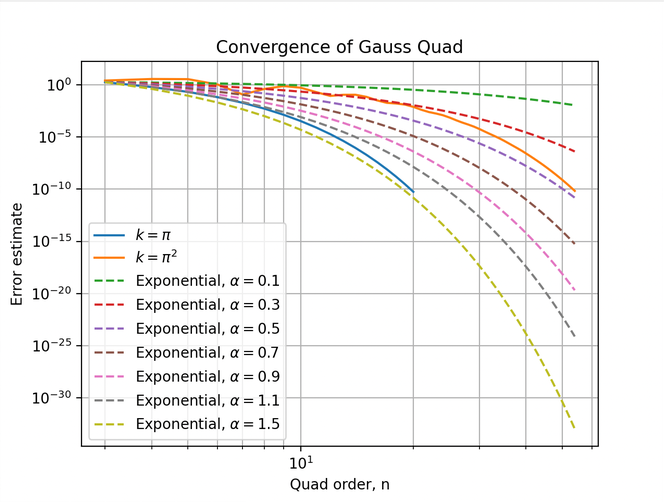
\includegraphics[width=0.75\linewidth]{exp_quad.png}
    \caption{Gauss Quadrature convergence compared with several exponential reference curves using different values of $\alpha$.}
    \label{fig:gauss-alpha-experiment}
\end{figure} 

The experimental curves demonstrate that a single value of $\alpha$ does not describe both cases equally well. The $k = \pi$ error decreases substantially faster than the $k = \pi^2$ error. Smaller values such as $\alpha = 0.1 $ and $0.3$ decrease too slowly to represent the $k = \pi$ data, while the large values more closely reproduce its rapid decay. In contrast, the $k = \pi^2$ results are better represented by a smaller value of $\alpha$. \\\\

An intermediate comparison was then made using $\alpha = 0.5$ and $\alpha = 1.5$. Initially, these reference rates were associated with the opposite data sets, as show in Figure~\ref{fig:gauss-before-appropriate-data-sets}. The $\alpha = 0.5$ reference decreases too slowly relative to the $k = \pi$ results, while the $\alpha = 1.5$ reference decreases much too rapidly relative to the $k = \pi^2$ results. This indicated that the two reference rates should instead be exchanged. 

\begin{figure}[H]
    \centering
    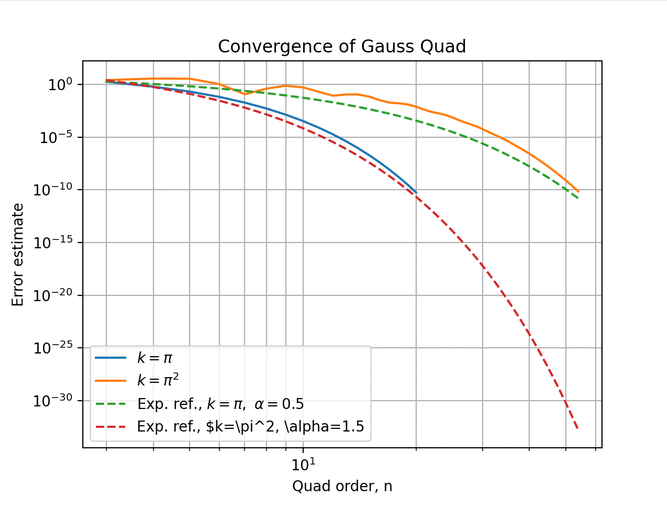
\includegraphics[width=0.75\linewidth]{aftExp_quad.png}
    \caption{Intermediate exponential reference curves before the fitted $\alpha$ values were associated with the appropriate data sets.}
    \label{fig:gauss-before-appropriate-data-sets}
\end{figure} 

The final comparison is shown in Figure~\ref{fig:gauss-final}. An exponential reference curve with 

\begin{equation}
    C = e, \space \alpha = 1.5
\end{equation}
was used for the $k = \pi$ case, while \begin{equation}
    C = e, \alpha = 0.5
\end{equation}
was used for the $k = \pi^2$ case. Each reference curve was plotted only over the range of quadrature orders associated with its corresponding numerical data. 
\begin{figure}[H]
    \centering
    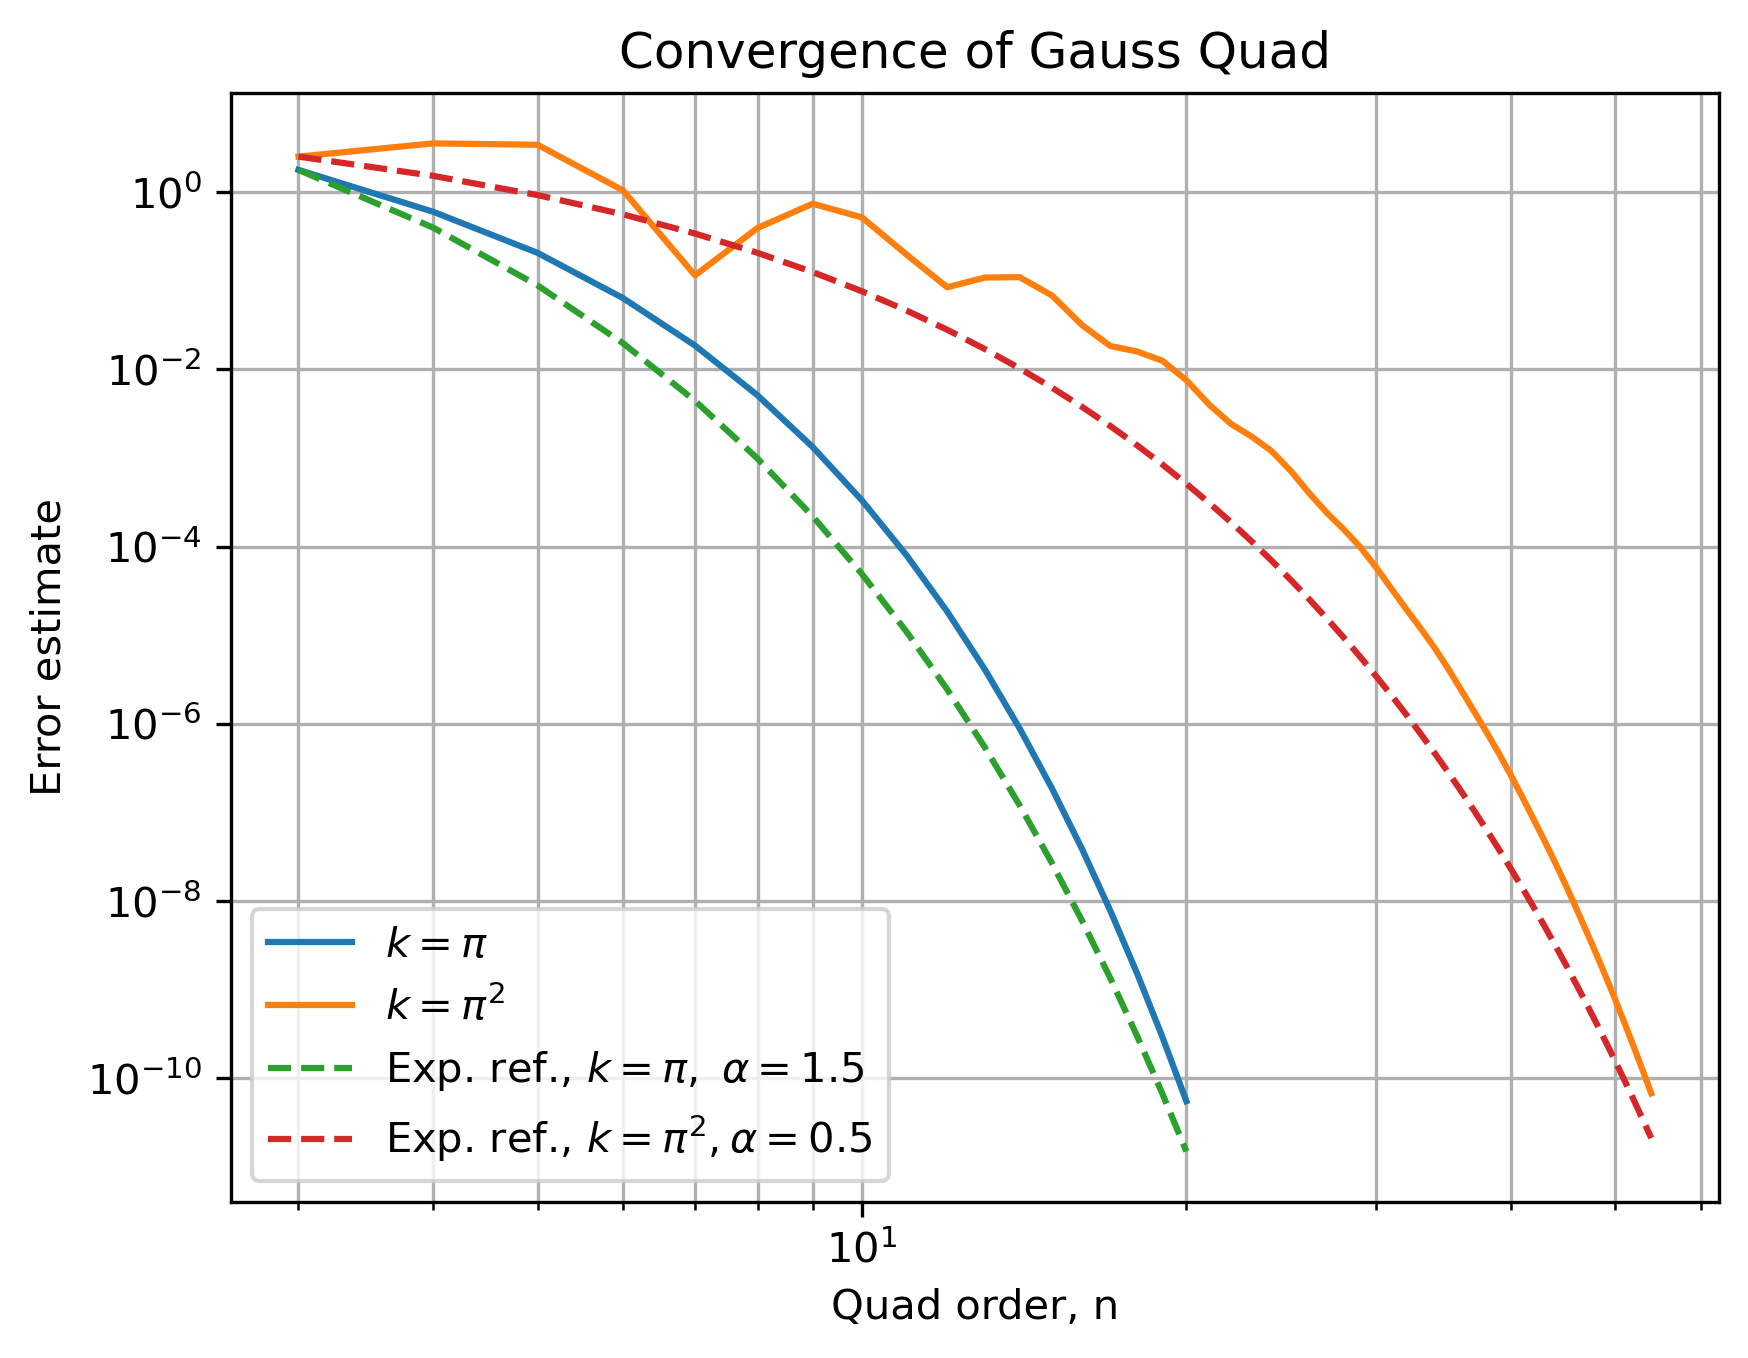
\includegraphics[width=0.75\linewidth]{gauss_converg.png}
    \caption{Final Gauss Quadrature convergence results with fitted exponential reference curves for $k = \pi$ and $k = \pi^2$.}
    \label{fig:gauss-final}
\end{figure} 
The final reference curves follow the general decay of their corresponding numerical results reasonably well. In particular, the $\alpha = 1.5$ reference reflects the faster decrease observed for $k = \pi$, while the $\alpha = 0.5$ reference more closely follows the slower $k = \pi^2$ case. The reference curves are not expected to pass through every numerical value, especially at small $n$, but their overall behavior supports the conclusion that the Gauss Quadrature errors decrease exponentially with increasing quadrature order.\\\\
Therefore, the numerical experiment is consistent with the expected convergence behavior \begin{equation}
    \epsilon(n) \sim C^{-\alpha n},
\end{equation}
although the observed value of $\alpha$ differs between the two choice of $k$.
\newpage
\section{2D Trapezoid Rule and 2D Finite Differencing in Cartesian and Curvilinear Coordinates}

\subsection{Method}
We were then tasked with estimating the values of integrals over two dimensions, involving transformations from the (r, s) curvilinear reference domain into cartesian coordinates. We were provided with skeleton code that plotted these domains, as well as a structure for our implementation of the 2D trapezoid method. 
The three domains considered were defined through transformations from the reference domain $\Omega_R=[-1,1]\times[-1,1]$. For the reference domain, the transformation was the identity
\begin{equation}
    x=r,\qquad y=s,
\end{equation}
with the determinant of its Jacobian
\begin{equation}
    J_0(r,s)
    =
    \det
    \begin{pmatrix}
        1 & 0\\
        0 & 1
    \end{pmatrix}
    =1.
\end{equation}
 
\noindent The second domain, $\Omega_1$, was obtained using the transformation
\begin{equation}
    x=r+0.1s,\qquad y=s,
\end{equation}
which produces a sheared version of the reference square, tilting the x coordinates to the right. Its Jacobian determinant is
\begin{equation}
    J_1(r,s)
    =
    \det
    \begin{pmatrix}
        1 & 0.1\\
        0 & 1
    \end{pmatrix}
    =1.
\end{equation}

\noindent The third domain, $\Omega_2$, was defined by the nonlinear transformation
\begin{equation}
    \begin{aligned}
        x &= \left(2+r+0.2\sin(5\pi s)\right)
        \cos\left(\frac{\pi s}{2}\right),\\
        y &= \left(2+r+0.2\sin(5\pi s)\right)
        \sin\left(\frac{\pi s}{2}\right).
    \end{aligned}
\end{equation}
Letting $R=2+r+0.2\sin(5\pi s),$ and $ \theta=\frac{\pi s}{2}$, we then found the Jacobian matrix of this transformation by hand and confirmed it using a computer algebra system. 
\begin{equation}
    \frac{\partial(x,y)}{\partial(r,s)}
    =
    \begin{pmatrix}
        \cos(\theta) &
        \pi\cos(5\pi s)\cos(\theta)
        -\dfrac{\pi}{2}R\sin(\theta)\\[6pt]
        \sin(\theta) &
        \pi\cos(5\pi s)\sin(\theta)
        +\dfrac{\pi}{2}R\cos(\theta)
    \end{pmatrix}.
\end{equation}
We calculated the determinant of this matrix, denoted $J_2$, by hand as well.
\begin{align}
    J_2(r,s) = \frac{\pi}{2}
       \left(2+r+0.2\sin(5\pi s)\right).
\end{align}

For each transformation, the integral over the physical domain was first converted to an integral over the reference domain using the corresponding transformation and Jacobian determinant. The code generated $n$ evenly spaced points in both the $r$ and $s$ directions and used these points to construct a 2D grid over the reference domain. Each point on this grid was then mapped to its corresponding $(x,y)$ coordinate using the specified transformation. The function was evaluated at these transformed coordinates and multiplied by the absolute value of the Jacobian determinant to account for any expansion or contraction of the volume beneath the transformed surface. The resulting values were then summed using the two-dimensional trapezoidal rule. Interior grid points were given full weight, points along an edge were given half weight, and corner points were given quarter weight. Finally, the weighted sum was multiplied by the square of the grid spacing to obtain the numerical approximation of the integral.
\\
Three functions were integrated over the two simplest transformed domains, $\Omega_1$ and $\Omega_R$. The first was the constant function
\begin{equation}
    u_1(x,y)=1,
\end{equation}
followed by the trigonometric function
\begin{equation}
    u_2(x,y)=\sin(x)\cos(y),
\end{equation}
and the exponential function
\begin{equation}
    u_3(x,y)=e^{x+y}.
\end{equation}
The goal was to determine how the results of our integration might change over the different domains, if at all, for three distinct values of $n$. That is, three distinct numbers of grid points. We anticipated that as $n$ increased, the accuracy of the method would as well. \\\\
% start of part 2 #5
For the final convergence experiment, we approximated the first partial derivatives of $u_2$ and $u_3$ on the transformed domain $\Omega_2$. The assignment specifies first-order forward finite differencing, \begin{equation}
    \hat{u_x}(x,y,h) = \frac{u(x+h,y) - u(x,y)}{h},
\end{equation}
and \begin{equation}
    \hat{u_y}(x,y,h) = \frac{u(x, y+h) - u(x,y)}{h},
\end{equation}
For \begin{equation}
    u_2(x,y) = sin(x) cos(y),
\end{equation}
the exact partial derivatives are \begin{equation}
    u_{2,x}(x,y)=cos(x)cos(y),
\end{equation}
and \begin{equation}
    u_{2,y}(x,y) = -sin(x)sin(y).
\end{equation}
Similarly, for \begin{equation}
    u_3(x,y) = e^{x+y},
\end{equation}
the exact derivatives are \begin{equation}
    u_{3,x}(x,y)=e^{x+y}, \quad  u_{3,y}(x,y)=e^{x+y}.
\end{equation}
The numerical derivatives were compared with these exact derivatives using the error expression specificied by the assignment, \begin{equation}
    f(x,y) = (\hat{u}_x - u_{x,exact} + \hat{u}_y - u_{y,exact})^2.
\end{equation}
This error function was then integrated over $\Omega_2$ using the previously implemented two-dimensional trapezoidal rule and the transformation $T_2$. the resulting error measure was \begin{equation}
    err(h) = \left(\int_{\Omega_2}f(x,y)dxdy\right)^{1/2}.
\end{equation}
The experiment was performed for \begin{equation}
    n = 8,16,32,64,128,256,
\end{equation}
where the grid spacing was determined by \begin{equation}
    h = \frac{2}{n-1}.
\end{equation}
For each value of $n$, the error was computed for both $u_2$ and $u_3$. The numerical results were then compared with reference curves proportional to $O(h)$ and $O(h^2)$. Since first-order forward finite differencing was used, the expected convergence rate was $O(h)$. 


\subsection{Interpretation}
Below is the result of our experiment in question 4A. 

\begin{table}[H]
    \centering
    \caption{Comparison of the integral approximations of $u_1$ over $\Omega_R$ and $\Omega_1$.}
    \label{tab:Question 4a}
    \begin{tabular}{c|cc}
        $n$ & $\Omega_R$ & $\Omega_1$ \\
        \hline
        \input{q4a_table.txt}
    \end{tabular}
\end{table}
Because we are integrating the constant function $u(x,y) = 1$, and the determinant of the Jacobian of both transformations to the domains $\Omega_1$ and $\Omega_R$ is 1, there is no change to the area of the non transformed domain to account for in the integration, and as such, the result does not change.
\\
For question 4B, we were asked to compute the integral of $u_2(x,y)=\sin(x)\cos(y)$ for three different values of $n$. The table below contains the results.
\begin{table}[H]
    \centering
    \caption{Comparison of the integral approximations of $u_2$ over $\Omega_R$ and $\Omega_1$.}
    \label{tab:Question 4b}
    \begin{tabular}{c|cc}
        $n$ & $\Omega_R$ & $\Omega_1$ \\
        \hline
        \input{q4b_table.txt}
    \end{tabular}
\end{table}
The expected value for the integral is indeed zero. This is because the function is odd in x, and we are integrating over a symmetrical interval. That is, 
\begin{equation}
    sin(-x) = -sin(x)
\end{equation}
\begin{equation} 
cos(-y) = cos(y) 
\end{equation}
and therefore
\begin{equation}
    sin(-x)cos(-y) = -sin(x)cos(y)
\end{equation}
As such, we expected the contributions from either side of the interval to cancel each other out. The reason for the very small nonzero values for the larger $n$ is likely floating point rounding errors. As can be seen in the table, these errors are of the order $10^{-16}$, where machine epsilon for 64 bit floating point is approximately $2.22 \times 10^{-16}$. Therefore, we believe that small differences in the computer's floating point representation and evaluation of the integrand at opposite sides of the domain prevented the contributions from canceling exactly, resulting in a small residual on the order of floating point precision.\\

For the convergence study in Question 5, we computed the numerical derivative error for $u_2$ and $u_3$ on $\Omega_2$ for the prescribed values of $n$. The resulting grid spacings and errors are shown in Table~\ref{tab:q5-errors}.
\begin{table}[H]
    \centering
    \caption{Numerical derivative errors for $u_2$ and $u_3$ on $\Omega_2$.}
    \label{tab:q5-errors}
    \begin{tabular}{c|c|c|c}
    $n$ & $h$ & $\mathrm{err}_{u_2}(h)$ & $\mathrm{err}_{u_3}(h)$ \\
    \hline 
    8   & 2.8571428571e-01 & 4.9614152024e-01 & 2.1592222574e+01 \\
    16  & 1.3333333333e-01 & 2.3221008088e-01 & 9.4355235497e+00 \\
    32  & 6.4516129032e-02 & 1.1237533659e-01 & 4.4439802485e+00 \\
    64  & 3.1746031746e-02 & 5.5292937054e-02 & 2.1609644466e+00 \\
    128 & 1.5748031496e-02 & 2.7426907540e-02 & 1.0660362058e+00 \\
    256 & 7.8431372549e-03 & 1.3659086671e-02 & 5.2950182080e-01 \\
    \end{tabular}
\end{table}
To determine the observed convergence rate, the errors were plotted against the grid spacing $h$ on logarithmic scales. The reference curves for first-order $O(h)$ convergence and second-order $O(h^2)$ convergence were included for comparison. 

\begin{figure}[H]
    \centering
    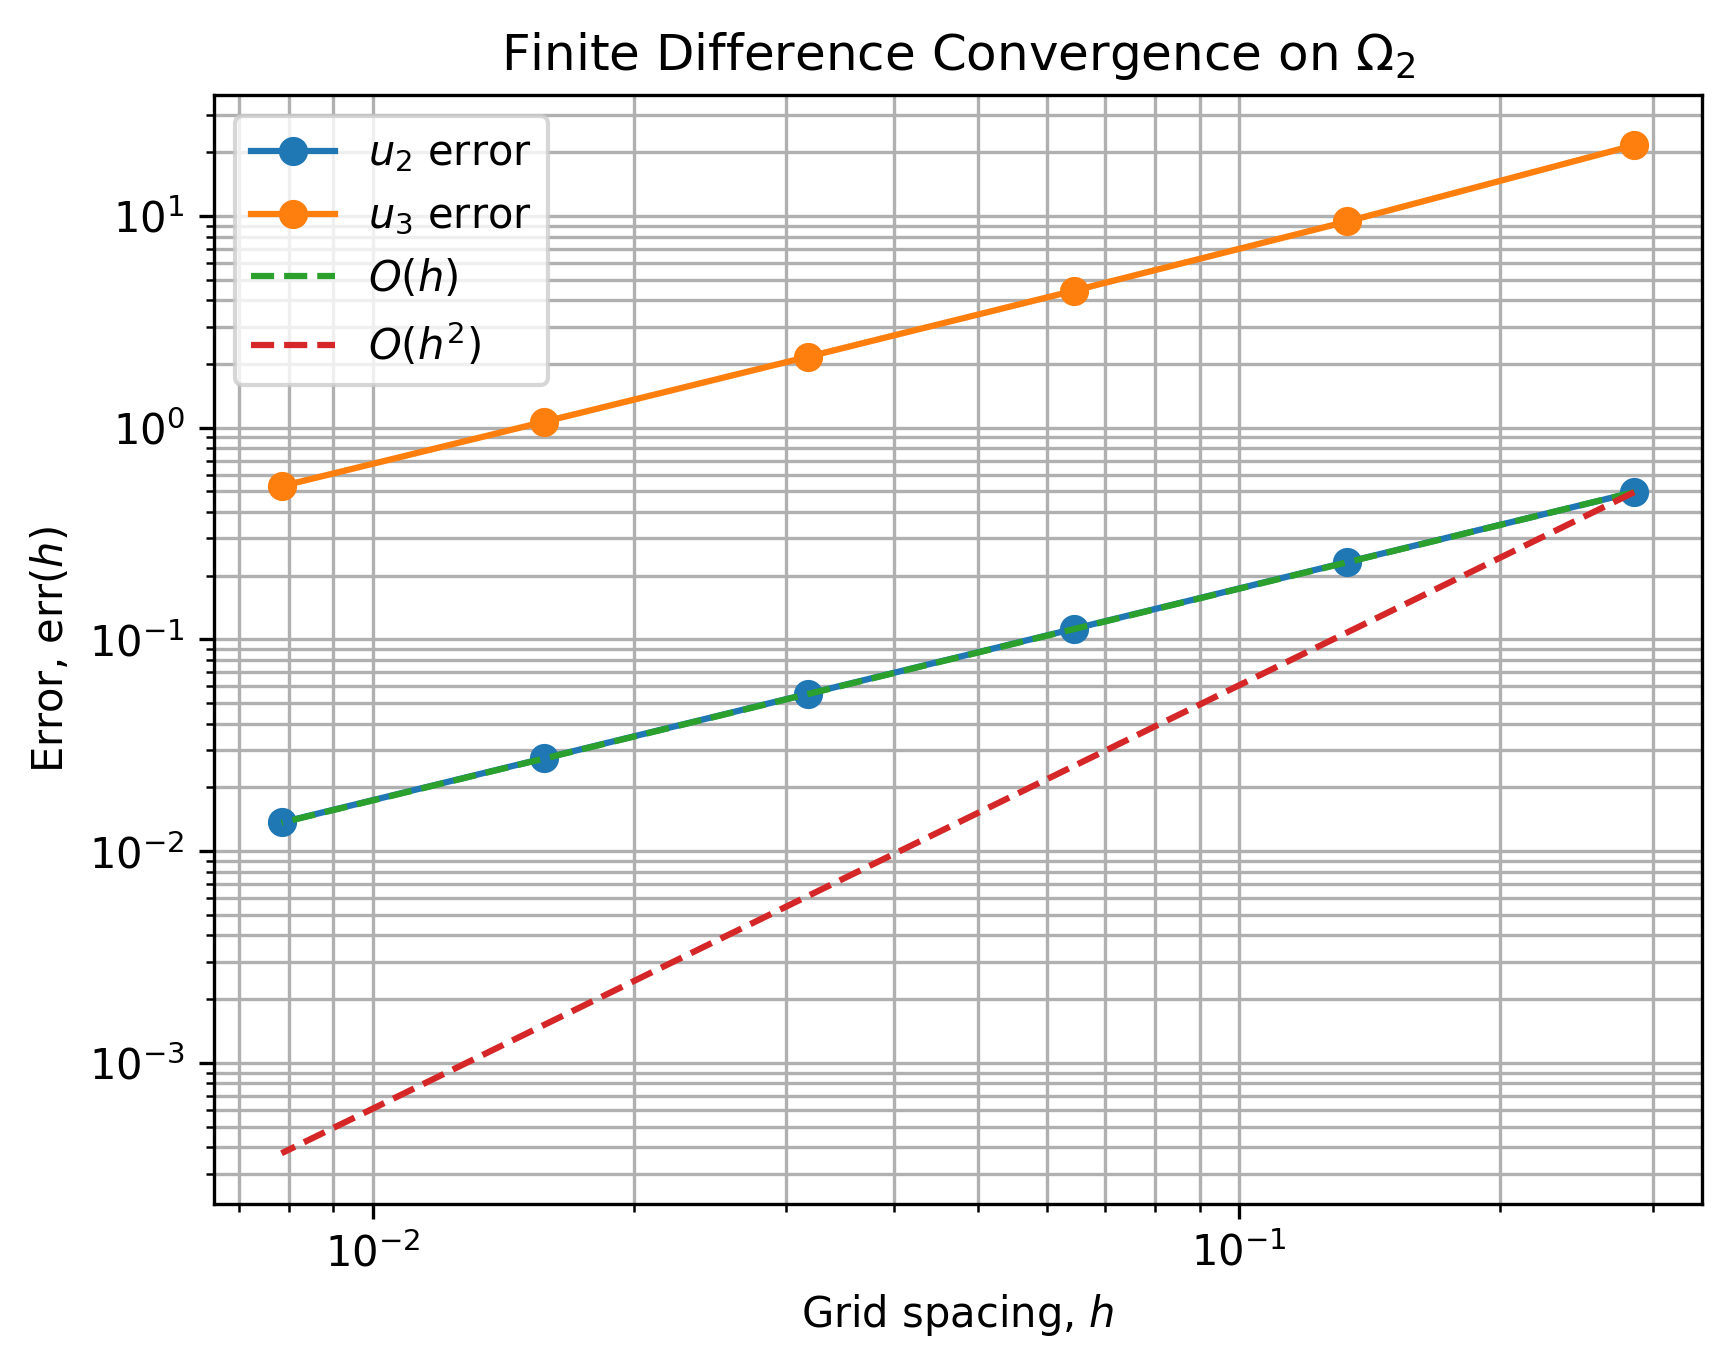
\includegraphics[width=0.8\textwidth]{error_on_omega2.png}
    \caption{Numerical derivative error for $u_2$ and $u_3$ on $\Omega_2$, compared with $O(h)$ and $O(h^2)$ reference curves.}
    \label{fig:omega2-error}
\end{figure}

The results in Figure~\ref{fig:omega2-error} show that the numerical derivative errors for both $u_2$ and $u_3$ decrease at, approximately, a first-order rate. The $O(h)$ reference curve nearly overlaps the $u_2$ error curve, providing particularly strong visual evidence of first-order convergence. The $u_3$ error is larger in magnitude, but its slope is also much more similar to the $O(h)$ reference curve than to the $O(h^2)$ reference curve. \\
This behavior is also visible in Table~\ref{tab:q5-errors}. As the grid spacing $h$ is reduced, the errors for both functions decrease by approximately the same factor. Therefore, the numerical results are consistent with \begin{equation}
    err(h) = O(h).
\end{equation}
This agrees with the expected theoretical convergence rate of the first-order forward finite-difference approximations used for the partial derivatives. Although the errors for $u_3$ are considerably larger than those for $u_2$, the magnitude of the error does not determine the order of convergence. The important observation is that both error curves decrease with approximately the same first-order dependence on $h$.

\end{document}  
